%%%%%%%%%%%%%%%%%%%%%%%%%%%%%%%%%%%%%%%%%%%%%%%%%%%%%%%%%%%%%%%%%%%%%%
% How to use writeLaTeX: 
%
% You edit the source code here on the left, and the preview on the
% right shows you the result within a few seconds.
%
% Bookmark this page and share the URL with your co-authors. They can
% edit at the same time!
%
% You can upload figures, bibliographies, custom classes and
% styles using the files menu.
%
%%%%%%%%%%%%%%%%%%%%%%%%%%%%%%%%%%%%%%%%%%%%%%%%%%%%%%%%%%%%%%%%%%%%%%

\documentclass[12pt]{article}

\usepackage{sbc-template}

\usepackage{graphicx,url}

%\usepackage[brazil]{babel}   
\usepackage[utf8]{inputenc}  

\usepackage{hyperref}

     
\sloppy

\title{Problema de Data Comum em Máquina Única Restrita}
% Decidir se vai ser Crew Scheduling ou Common due date scheduling

\author{João Victor Lagos\inst{1}, Daniel José\inst{1}, Felipe Vahia\inst{1}}


\address{Instituto de Computação -- Universidade Federal Fluminense (IC/UFF)\\
  Caixa Postal 24.220-900 -- Niterói -- RJ -- Brazil
\nextinstitute
  Departmento de Ciência da Computação -- Universidade Federal Fluminense (UFF)\\
  Rio de Janeiro, BR.
  \email{\{joaolagos,danieljms,felipevahia\}@id.uff.br}
}

\begin{document} 

\maketitle
     
\begin{resumo} 
Este trabalho explora o Problema de Data Comum em Máquina Única Restrita, um problema clássico de otimização combinatória. O objetivo é agendar tarefas, com tempos de processamento determinados, em uma única máquina, de forma a minimizar a soma das penalidades de antecipação e atraso em relação a uma data comum. Para cada tarefa, as penalidades são aplicadas conforme o término ocorre antes ou depois da data. Foram desenvolvidos dois algoritmos meta-heurísticos baseados em Simulated Annealing e Busca Tabu para resolver o problema. Os resultados incluem a calibração de parâmetros, o valor médio das soluções em 10 execuções, a melhor solução encontrada em 10 execuções e o tempo médio computacional necessário para essas execuções.
\end{resumo}

\begin{abstract}  
This work explores the Restricted Single-Machine Common Due Date Problem, a classic combinatorial optimization problem. The goal is to schedule tasks with deterministic processing times on a single machine to minimize the sum of earliness and tardiness penalties relative to a common due date. For each task, penalties are incurred depending on whether the completion occurs before or after the due date. Two heuristic algorithms based on Simulated Annealing and Tabu Search were developed to solve the problem. The results include parameter calibration, the average solution value over 10 runs, the best solution found in 10 runs, and the average computational time required for these executions.  
\end{abstract}



\section{Introdução}

\section{O Problema: Common Due Date Scheduling} \label{sec:o_problema}

O problema de agendamento com data de vencimento comum restrita em uma máquina única foi obtido através do \href{https://people.brunel.ac.uk/~mastjjb/jeb/orlib/schinfo.html}{OR Library - Common Due Date Scheduling} e pode ser definido da seguinte maneira:

Dado um conjunto de $n$ tarefas com tempos de processamento determinísticos $p(i)$ e uma data de vencimento comum $d$, todas as tarefas devem ser processadas em uma única máquina. Para cada tarefa $i$, são atribuídas penalidades individuais de adiantamento $a(i)$ e de atraso $b(i)$. Essas penalidades são aplicadas caso a tarefa seja concluída antes ou depois da data de vencimento $d$, respectivamente. O objetivo é determinar uma sequência de execução das $n$ tarefas que minimize a soma total das penalidades de adiantamento e atraso.

Ou seja, em resumo, deve-se obter a ordem ou sequência em que os trabalhos (jobs) devem ser processados pela máquina para minimizar as penalidades totais, considerando antecipações e atrasos.

No problema descrito, tem-se os seguintes elementos:

\begin{itemize}
\item \textbf{$n$ trabalhos}: Cada trabalho $i$ tem um tempo de processamento $p(i)$, uma penalidade de antecipação $a(i)$ e uma penalidade de atraso $b(i)$.
\item \textbf{Data de vencimento comum} $d$: Calculada com base na soma total dos tempos de processamento do problema multiplicada por um fator $h$ (restritivo ou não), conforme a  
\item \textbf{Objetivo}: Encontrar a sequência de tarefas que minimiza a soma das penalidades de antecipação e atraso para todos os trabalhos.
\end{itemize}


O formato interno dos arquivos de dados utilizados para esse problema segue a seguinte estrutura:

\begin{itemize}
    \item A primeira linha contém o número total de problemas.
    \item Para cada problema subsequente:
    \begin{itemize}
        \item A primeira linha especifica o número de trabalhos ($n$) associados ao problema.
        \item As $n$ linhas seguintes contêm três valores por linha: 
        \begin{itemize}
            \item $p(i)$: Tempo de processamento do trabalho $i$.
            \item $a(i)$: Penalidade por antecipação do trabalho $i$.
            \item $b(i)$: Penalidade por atraso do trabalho $i$.
        \end{itemize}
    \end{itemize}
\end{itemize}

Exemplo visual do formato de um arquivo de dados:

\begin{verbatim}
10                    # Número total de problemas
10                    # Número de trabalhos (n) para Problema 1
20  4  5              # p(i): temp. procss, a(i): pen. antecipação, b(i): pen. por atraso
..  .. ..
13 10  1              # Exemplos subsequentes para o mesmo problema
..  .. ..
10                    # Número de trabalhos (n) para o último problema
16  2  6
..  .. ..
11  1 12
\end{verbatim}

\subsection{Exemplo Simplificado}

Suponha que você tenha 3 trabalhos com os seguintes dados:  

$p(1) = 5$, $a(1) = 2$, $b(1) = 3$  

$p(2) = 3$, $a(2) = 1$, $b(2) = 4$  

$p(3) = 4$, $a(3) = 5$, $b(3) = 2$  

$h = 0.6$

A data de vencimento comum $d$ é calculada como:  
\[
d = 0.6 \times SOMA\_P = 0.6 \times (5 + 3 + 4) = 7
\]

Neste exemplo, você precisa determinar uma ordem de execução das tarefas (por exemplo, [1, 2, 3], [2, 3, 1], etc.) que minimize a soma das penalidades totais. A penalidade de cada trabalho depende se ele termina antes ou depois da data de vencimento $d$:
\begin{itemize}
    \item Penalidade por antecipação ($a(i)$) é aplicada se o trabalho termina antes de $d$.
    \item Penalidade por atraso ($b(i)$) é aplicada se o trabalho termina após $d$.
\end{itemize}
O desafio consiste em encontrar a sequência que resulta no menor custo total de antecipações e atrasos.

\subsection{Função Objetivo} \label{subsec:funcao_objetivo}

A função objetivo para o problema de agendamento com data de vencimento comum em máquina única busca minimizar a soma total das penalidades de antecipação e atraso de todas as tarefas. Dada uma sequência de execução dos $n$ trabalhos, a função objetivo pode ser definida como:

\[
C = \sum_{i=1}^{n} \left[ a(i) \max(0, d - C_i) + b(i) \max(0, C_i - d) \right]
\]

onde:  
\begin{itemize}
    \item $C_i$ é o instante de conclusão do trabalho $i$ na sequência dada.  
    \item $d$ é a data de vencimento comum calculada para todas as tarefas.  
    \item $a(i)$ e $b(i)$ são as penalidades individuais de antecipação e atraso, respectivamente, para o trabalho $i$.  
    \item $\max(0, d - C_i)$ representa o tempo de antecipação (se existir), e $\max(0, C_i - d)$ representa o tempo de atraso (se existir).
\end{itemize}

O objetivo é encontrar a melhor sequência de execução dos trabalhos que minimize o valor de $C$, garantindo a menor soma de custos associados ao adiantamento e ao atraso das tarefas.

\section{As Duas Meta-heurísticas} \label{sec:metaheuristicas}

Para resolver o problema de agendamento com data de vencimento comum em máquina única, foram implementadas duas meta-heurísticas populares: Busca Tabu (Tabu Search) e Simulated Annealing. Essas abordagens são amplamente utilizadas para encontrar soluções aproximadas em problemas de otimização combinatória complexos devido à sua capacidade de escapar de ótimos locais e explorar o espaço de soluções de maneira eficiente.

Vale lembrar que a solução inicial foi feita a partir de uma heurística construtiva aleatória.

\subsection{Busca Tabu}

A Busca Tabu é uma meta-heurística baseada em memória que guia a exploração do espaço de soluções, evitando a revisitação de soluções já analisadas. Para isso, utiliza uma estrutura de memória chamada \textit{lista tabu}, que armazena movimentos ou soluções proibidas temporariamente. O algoritmo Busca Tabu implementado neste trabalho utiliza os seguintes componentes principais:

\begin{itemize}
    \item \textbf{Solução Inicial}: Uma sequência inicial de execução das tarefas, gerada aleatoriamente ou por heurísticas simples.
    \item \textbf{Movimentos}: Trocas ou reordenações de tarefas para gerar novas soluções candidatas.
    \item \textbf{Lista Tabu}: Armazena soluções recentes para evitar ciclos e melhorar a exploração global.
\end{itemize}

O pseudocódigo para o Busca Tabu está ilustrado abaixo:

\begin{figure}[h]  
    \centering 
    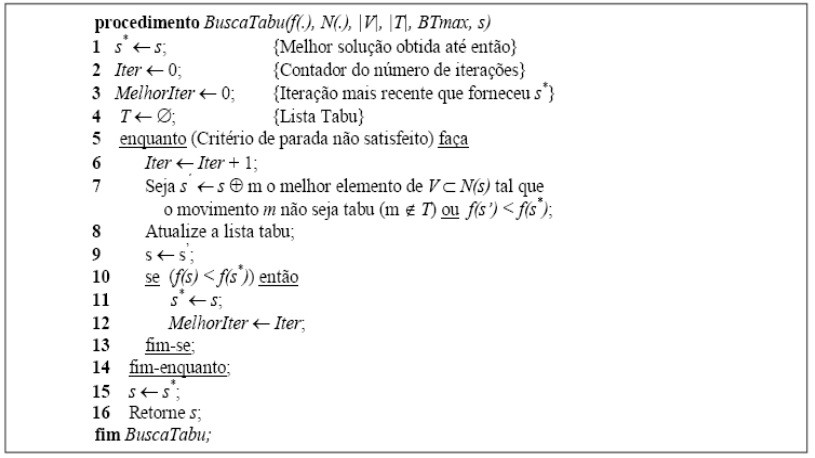
\includegraphics[width=1\textwidth]{busca_tabu.jpg}  
    \caption{Pseudocódigo do Busca Tabu}  % Legenda da imagem
    \label{fig:busca_tabu}  % Etiqueta para referenciar a imagem
\end{figure}


O objetivo é continuar explorando novas soluções, escapando de ótimos locais e melhorando iterativamente a solução atual.

\subsection{Simulated Annealing}

O Simulated Annealing é inspirado no processo físico de recozimento, onde um material é aquecido e resfriado lentamente para minimizar sua energia interna. A meta-heurística segue uma abordagem probabilística para aceitar ou rejeitar soluções piores com base em uma função de temperatura decrescente, o que permite escapar de ótimos locais.

Os principais componentes do algoritmo implementado incluem:

\begin{itemize}
    \item \textbf{Solução Inicial}: Uma sequência de execução inicial das tarefas.
    \item \textbf{Temperatura Inicial}: Controla a probabilidade de aceitar soluções piores no início do processo.
    \item \textbf{Função de Decaimento}: Reduz gradualmente a temperatura durante a execução.
    \item \textbf{Critério de Aceitação}: Soluções melhores são sempre aceitas, enquanto soluções piores são aceitas com probabilidade $e^{-\Delta C / T}$, onde $\Delta C$ é a diferença de custo e $T$ é a temperatura atual.
\end{itemize}

O pseudocódigo para o Busca Tabu está ilustrado abaixo:

\begin{figure}[h]  
    \centering 
    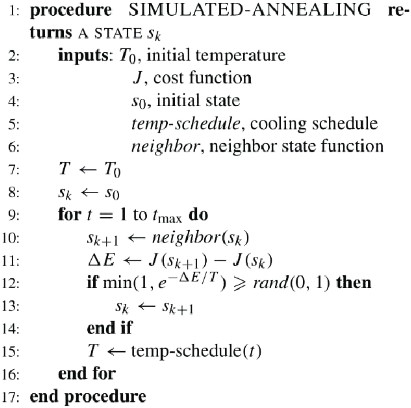
\includegraphics[width=0.6\textwidth]{busca_SA.jpg}  
    \caption{Pseudocódigo do Simulated Annealing}  % Legenda da imagem
    \label{fig:busca_SA}  % Etiqueta para referenciar a imagem
\end{figure}

A combinação de resfriamento controlado e exploração probabilística permite que o Simulated Annealing busque soluções próximas do ótimo global, evitando ficar preso em ótimos locais.



\section{Calibração de Parâmetros}

A calibração de parâmetros é uma etapa fundamental em muitos modelos e algoritmos, pois garante que os parâmetros ajustados ou escolhidos maximizem a performance ou a precisão do modelo. O objetivo principal dessa etapa é determinar os valores ótimos para os parâmetros do sistema de modo que ele se comporte de forma eficiente e produza resultados que estejam alinhados com as expectativas ou dados empíricos.

\subsection{Parâmetros no Busca Tabu}

Os parâmetros de importância para a meta-heurística Busca Tabu são o número de iterações máximas e o tamanho da lista Tabu. Esses parâmetros têm grande influência no desempenho e na capacidade de encontrar uma solução ótima ou quase ótima dentro de um espaço de busca.

\begin{itemize}
    \item \textbf{Número de iterações máximas:} Este parâmetro define o número máximo de iterações que o algoritmo irá realizar. Um número elevado de iterações permite que o algoritmo explore mais profundamente o espaço de soluções, aumentando as chances de encontrar uma solução melhor. No entanto, um número excessivo de iterações pode levar a um alto custo computacional sem melhorias significativas nos resultados.
    \begin{itemize}
        \item Nesse sentido, o valor para o referido parâmetro foi de \textbf{5.000 iterações} (max\_iter=5000).
    \end{itemize}
    
    \item \textbf{Tamanho da lista Tabu:} O tamanho da lista Tabu determina quantas soluções anteriores são lembradas. Um tamanho muito pequeno pode resultar em repetição de soluções e perda de diversidade na busca, enquanto um tamanho muito grande pode levar a uma exploração muito restrita do espaço de soluções.
    \begin{itemize}
        \item Nesse sentido, optamos por um tamanho de \textbf{10 soluções} (tamanho\_lista\_tabu=10).
    \end{itemize}
\end{itemize}

\subsection{Parâmetros no Simulated Annealing}

FAZER...


\section{Valor Médio da Solução (10 Execuções)}



\section{Melhor Solução (10 Execuções)}



\section{Tempo Médio Computacional (10 Execuções)}



\section{Conclusão}


\section{Figures and Captions}\label{sec:figs}


Figure and table captions should be centered if less than one line
(Figure~\ref{fig:exampleFig1}), otherwise justified and indented by 0.8cm on
both margins, as shown in Figure~\ref{fig:exampleFig2}. The caption font must
be Helvetica, 10 point, boldface, with 6 points of space before and after each
caption.

\begin{figure}[ht]
\centering
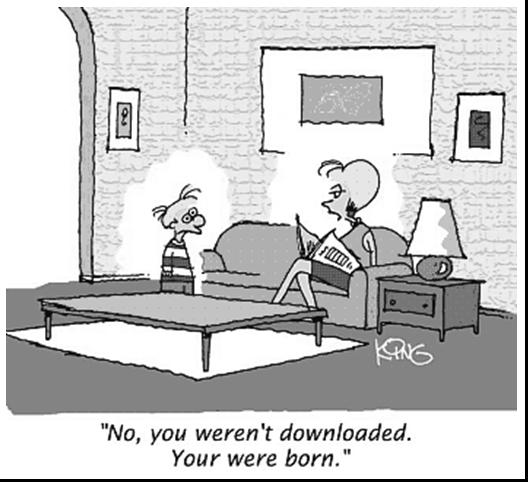
\includegraphics[width=.5\textwidth]{fig1.jpg}
\caption{A typical figure}
\label{fig:exampleFig1}
\end{figure}

\begin{figure}[ht]
\centering
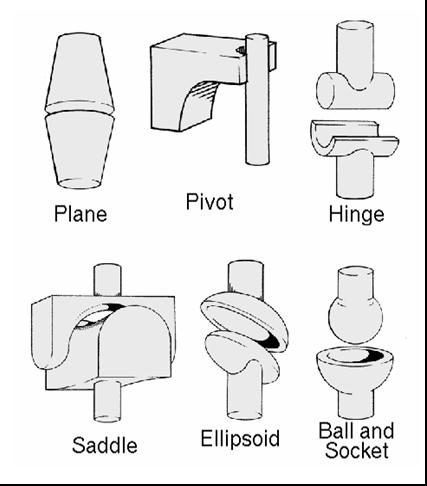
\includegraphics[width=.3\textwidth]{fig2.jpg}
\caption{This figure is an example of a figure caption taking more than one
  line and justified considering margins mentioned in Section~\ref{sec:figs}.}
\label{fig:exampleFig2}
\end{figure}

In tables, try to avoid the use of colored or shaded backgrounds, and avoid
thick, doubled, or unnecessary framing lines. When reporting empirical data,
do not use more decimal digits than warranted by their precision and
reproducibility. Table caption must be placed before the table (see Table 1)
and the font used must also be Helvetica, 10 point, boldface, with 6 points of
space before and after each caption.

\begin{table}[ht]
\centering
\caption{Variables to be considered on the evaluation of interaction
  techniques}
\label{tab:exTable1}
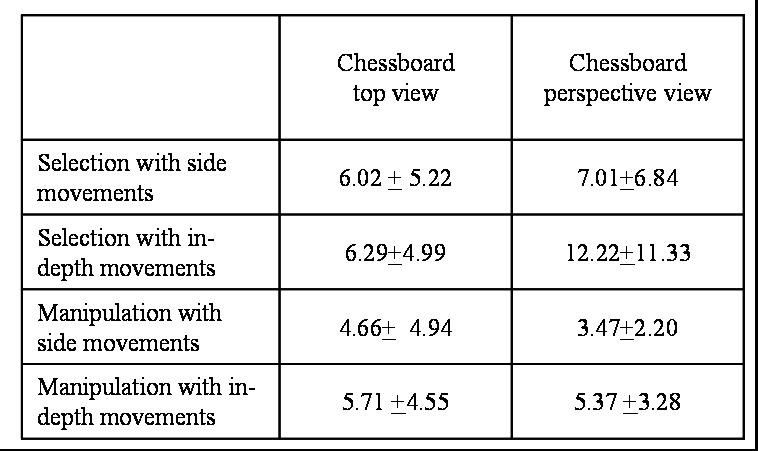
\includegraphics[width=.7\textwidth]{table.jpg}
\end{table}

\section{Images}

\section{References}

Bibliographic references must be unambiguous and uniform.  We recommend giving
the author names references in brackets, e.g. \cite{knuth:84},
\cite{boulic:91}, and \cite{smith:99}.

The references must be listed using 12 point font size, with 6 points of space
before each reference. The first line of each reference should not be
indented, while the subsequent should be indented by 0.5 cm.

\bibliographystyle{sbc}
\bibliography{sbc-template}

\end{document}
